\documentclass[12pt, twoside]{article}
\usepackage[letterpaper, margin=1in, headsep=0.5in]{geometry}
\usepackage[english]{babel}
\usepackage[utf8]{inputenc}
\usepackage{amsmath}
\usepackage{amsfonts}
\usepackage{amssymb}
\usepackage{tikz}
%\usetikzlibrary{quotes, angles}

\usepackage{graphicx}
\usepackage{enumitem}
\usepackage{multicol}

\usepackage{fancyhdr}
\pagestyle{fancy}
\fancyhf{}
\renewcommand{\headrulewidth}{0pt} % disable the underline of the header

\fancyhead[RE]{\thepage}
\fancyhead[RO]{\thepage \\ Name: \hspace{3cm}}
\fancyhead[L]{BECA / Dr. Huson / 10th Grade Geometry\\* 8 January 2019}

\begin{document}
\subsubsection*{Do Now: Constructions practice}
 \begin{enumerate}

   \item Using a compass and straightedge, construct the angle bisector of $\angle B$, one of the vertices of the rhombus $ABCD$.\vspace{2cm}
       \begin{center}
       \begin{tikzpicture}[scale=.6]
         %\draw [thick, <->] (-7.4,0) -- (10.4,0) node [right] {$x$};
         %\draw [thick, <->] (0,-6.4)--(0,10.4) node [above] {$y$};
         \draw [thick]
         (0,0) node[below left] {$A$}--
         (5,12) node[left] {$B$}--
         (18,12) node[below right] {$C$}--
         (13,0) node[below right] {$D$}--cycle;

       \end{tikzpicture}
     \end{center} \vspace{2cm}

     \item Using a compass and straightedge, construct a line segment $\overline{AC}$ on the ray $\overrightarrow{AB}$ that is twice the length of $\overline{AB}$.\vspace{3cm}
         \begin{center}
         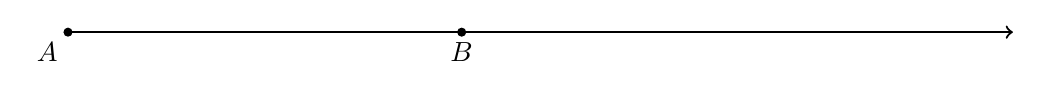
\begin{tikzpicture}
           %\draw [thick, <->] (-7.4,0) -- (10.4,0) node [right] {$x$};
           %\draw [thick, <->] (0,-6.4)--(0,10.4) node [above] {$y$};
           \draw [thick, ->]
           (0,0) node[below left] {$A$}--
           (5,0) node[below] {$B$}--
           (12,0);
           \draw [fill] (0,0) circle[radius=0.05];
           \draw [fill] (5,0) circle[radius=0.05];
         \end{tikzpicture}
       \end{center}

  \newpage

  \item Using a compass and straightedge, construct $M$, the midpoint of $\overline{AB}$. Then draw the median $\overline{CM}$.
  \vspace{2cm}
      \begin{center}
      \begin{tikzpicture}[scale=1.2]
        %\draw [thick, <->] (-7.4,0) -- (10.4,0) node [right] {$x$};
        %\draw [thick, <->] (0,-6.4)--(0,10.4) node [above] {$y$};

        \draw [thick]
        (5,-1) node[below left] {$A$}--
        (8,2) node[right] {$B$}--
        (1,0) node[below left] {$C$}--cycle;
      \end{tikzpicture}
    \end{center} \vspace{2cm}

    \item Using a compass and straightedge, dilate $\triangle ABC$ by a scale factor of 2 centered at $A$.\\[0.25cm] Construct line segment $\overline{AB'}$ that is twice the length of $\overline{AB}$ and $\overline{AC'}$ that is twice the length of $\overline{AC}$. Draw $\overline{A'B'}$ to complete the desired triangle, $\triangle AB'C'$. \vspace{2cm}
        \begin{center}
        \begin{tikzpicture}
          %\draw [thick, <->] (-7.4,0) -- (10.4,0) node [right] {$x$};
          %\draw [thick, <->] (0,-6.4)--(0,10.4) node [above] {$y$};
          \draw [thick, <->]
          (10,5)--
          (4,2) node[above left] {$C$}--
          (0,0) node[below left] {$A$}--
          (5,-1) node[below] {$B$}--
          (12,-2.4);
          \draw [thick] (4,2)--(5,-1);
          \draw [fill] (0,0) circle[radius=0.05];
          \draw [fill] (5,-1) circle[radius=0.05];
          \draw [fill] (4,2) circle[radius=0.05];
        \end{tikzpicture}
      \end{center}

  \newpage


\end{enumerate}
\end{document}
